\documentclass[svgnames]{beamer} % for xcolor https://latex.org/forum/viewtopic.php?t=2445 
\mode<presentation>
{
\usetheme{Warsaw}
\setbeamertemplate{page number in head/foot}[totalframenumber]
%\setbeamertemplate{footline}[frame number]
\setbeamertemplate{headline}{}
\setbeamercovered{transparent}
% or whatever (possibly just delete it)
}

\usepackage[english]{babel}
\usepackage[utf8]{inputenc}

\title{Matrix-free finite element method}
\institute[UH] {
	\includegraphicsw[.3]{logo_uh.png}
}
\date[December 10, 2019]{COSC\,6365 Final Project, December 10, 2019}

% bold for everything
\usepackage{bm}
% lowercase mathcal font
\usepackage{dutchcal}
\hypersetup{
	colorlinks,
	allcolors=.,
	urlcolor=blue,
	filecolor=blue
}
% braces for subeqns and boxes
\usepackage{empheq}
% http://mirror.hmc.edu/ctan/macros/latex/contrib/mathtools/empheq.pdf
\newcommand*\widefbox[1]{\fbox{\hspace{1em}#1\hspace{1em}}}
% hl
\usepackage{soul}
\makeatletter
\let\HL\hl
\renewcommand\hl{%
	\let\set@color\beamerorig@set@color
	\let\reset@color\beamerorig@reset@color
	\HL}
\makeatother
% sub figures / grids of pictures
\usepackage{subcaption} 
\graphicspath{{./img/}} % includegraphics path
\newcommand{\includegraphicsw}[2][1.]{\includegraphics[width=#1\linewidth]{#2}}
\newcommand{\svginput}[1]{\input{img/#1}} % pdf_tex path
\newcommand{\svginputw}[2][1.]{\def\svgwidth{#1\linewidth}\input{./img/#2}} % pdf_tex path
% tables
\let\oldtabular\tabular
\renewcommand{\tabular}[1][1.5]{\def\arraystretch{#1}\oldtabular}
\usepackage{hhline}
\usepackage{multirow}
% \coloneqq
\usepackage{mathtools}
% math commands for convinience
\DeclareMathOperator{\argmin}{arg\,min}
% bold vectors
\newcommand{\vect}[1]{\boldsymbol{\mathbf{#1}}}

\newcommand{\bcell}{T}
\newcommand{\bmesh}{{\vect{\mathcal T}}}
\newcommand{\mmesh}{{\vect{\mathcal \tau}}}
\newcommand{\bfaces}[1][]{{\vect{\mathcal F}_{\text{#1}}}}
\newcommand{\mfaces}[1][]{{\vect{\mathcal f}_{\text{#1}}}}

%\newcommand{\LTwo}{{\mathbb L^2}}
%\newcommand{\lTwo}{{\mathcal l^2}}
%\newcommand{\HDiv}{{\mathbb H_\text{div}}}
%\newcommand{\Rn}[1]{{\mathbb R^{#1}}}
%\newcommand{\Pn}[1]{{\mathbb P^{#1}}}
%\newcommand{\LTwoSpace}[1][\Omega]{{\mathbb L^2\left({#1}\right)}}
%\newcommand{\HSpace}[1]{{\mathbb H^{#1}\left(\Omega\right)}}
%\newcommand{\lTwoSpace}[1][\Omega]{{\mathcal l^2\left({#1}\right)}}
%\newcommand{\HDivSpace}[1][\Omega]{{\mathbb H_\text{div}\left({#1}\right)}}
%\newcommand{\PnSpace}[2]{{\mathbb P^{#1}\left({#2}\right)}}

% precond
\newcommand{\Pbd}{\mathbcal P_{\text{BD}}}
\newcommand{\Pbt}{\mathbcal P_{\text{BT}}}
\newcommand{\Pmg}{\vect P_{\text{MG}}}
\newcommand{\Pmgv}{\vect P_{\text{MG(V)}}}
\newcommand{\Pilu}{\vect P_{\text{ILU(0)}}}

\newcommand{\USpace}{\mathbb{\vect U}}
\newcommand{\PSpace}{\mathbb P}
\usepackage{dutchcal} % lowercase mathcal font
\newcommand{\aForm}[2]{\mathbcal a(#1, #2)}
\newcommand{\bForm}[2]{\mathbcal b(#1, #2)}
\newcommand{\lForm}[1]{\mathbcal l(#1)}
\newcommand{\LSpace}{\mathbb L^2}
\newcommand{\HSpace}{\mathbb H^1}

% differentials
\newcommand*\diff{\mathop{}\!\mathrm{d}}
\newcommand*\Diff[1]{\mathop{}\!\mathrm{d^#1}}

\usepackage{listings}
\definecolor{mygreen}{rgb}{0,0.6,0}
\lstset{
	%	language=C++,
	%	basicstyle=\footnotesize\ttfamily,
	breaklines=true,
	%	commentstyle=\color{mygreen},
	frame=l,
	xleftmargin=5pt,
	tabsize=2,
	%	belowskip=-1pt
} 

\begin{document}

	\author[K. Williams, A. Zhiliakov]{%
		\begin{tabular}[1.]{cc}
			Kyle Williams & Alexander Zhiliakov \\
			\href{mailto:kylew@math.uh.edu}{kylew@math.uh.edu} & \href{mailto:alex@math.uh.edu}{alex@math.uh.edu}
		\end{tabular}
		\vskip -1mm
	}

	\begin{frame}
		\titlepage
	\end{frame}

%	\begin{frame}{Overview}
%		\tableofcontents
%	\end{frame}
%	
%	\section{Theoretical background}

	\begin{frame}{Finite element method workflow \& motivation}
		\begin{enumerate}
			\item $L\,u = f$ + BCs $\Rightarrow$ Time discretization, linearization and finite element approximation $\Rightarrow$ Linear system~$\vect A\,\vect x = \vect b$ with \textbf{stiffness matrix}~$\vect A \in \mathbb R^{n\times n}$
			\item For big complex problems, especially in 3D, it is typical to use an iterative solver with a suitable preconditioner to solve the system
			\item The core operation is~$\vect x \mapsto \vect A\,\vect x \eqqcolon \vect z$
		\end{enumerate}
		\begin{figure}
			\begin{subfigure}{.5\linewidth}
				\centering
				\includegraphicsw[.8]{sparse.pdf}
				{Nonzero pattern of~$\vect A$}
			\end{subfigure}%
			\begin{subfigure}{.5\linewidth}
				$\vect A$ is \textbf{sparse}, i.e. it requires~$O(n)$ memory resources. Hence it is crucially important that the sparse matrix-vector multiplication is implemented efficiently.
			\end{subfigure}
		\end{figure}
	\end{frame}

	\begin{frame}{Stiffness matrix assembly}
		For~$L = -\nabla\cdot(\vect K\,\nabla)$ we have~$\vect A_{ij} = \int \vect K\,\nabla\phi_j\cdot\nabla\phi_i$ with $\phi_i$ being a basis function with a compact support; $\phi_i$ is typically chosen as a piecewise polynomial of degree~$k$.
		\begin{figure}
			\begin{subfigure}{.45\linewidth}
				\centering
				\includegraphicsw[.8]{mesh.png}
				Domain mesh
			\end{subfigure}%
			\begin{subfigure}{.55\linewidth}
				$\vect A$ is assembled from small cell matrices~$\vect A_\text{cell} \in \mathbb R^{k^{\text{dim}}\times k^{\text{dim}}}$. Formally it can be written as
				$$
					\vect A = \sum \vect P^T_\text{cell}\,\vect A_\text{cell}\,\vect P_\text{cell},
				$$
				where rectangular matrix~$\vect P_\text{cell}$ connect local cell d.o.f. to global mesh ones.
			\end{subfigure}
		\end{figure}
	\end{frame}	

	\begin{frame}[fragile]{Sparse matrix-vector multiplication}
		It is very common that $\vect A$ is represented in CSR format. In this case multiplication takes the form:
		\begin{lstlisting}[basicstyle=\small]
			for (size_t i = 0; i < nrows; ++i) 
				for (k = rowptr[i]; k < rowptr[i+1]; ++k)
					z[i] += val[k] * x[colind[k]];
		\end{lstlisting}
		CSR is optimal in the sense that both storage and multiplication require~$O(n)$ resources. However,
		\begin{enumerate}
			\item there is no spatial locality for~$\vect x$, and
			\item there are 5 memory refs vs. 2 arithmetic operations, i.e. the routine is memory bandwidth bounded
		\end{enumerate}
	\end{frame}	
	
	\begin{frame}{Matrix-free approach: Idea}
	The alternative approach is \textbf{matrix-free} implementation: Do not store the big sparse matrix~$\vect A$ but compute the action of its cell matrices~$\vect A_\text{cell}$ on the fly.
		\begin{enumerate}
			\item Low arithmetic intensity is the bottleneck for matrix-based computations; Matrix-free evaluation that reads less data can be advantageous even if it does more computations
			\item Matrix-free methods have a better complexity per degree of freedom:~$O(k)$ vs.~$O(k^\text{dim})$ for matrix-based methods ($k$ is basis func degree); This makes it attractive for higher order elements $k > 1$ and dim = 3~
\includegraphics[width=12px]{clown.png}
		\end{enumerate}
	\end{frame}	
	
	\begin{frame}{Matrix-free approach: Implementation}
		Our aim is to rewrite
		$$
			\vect x \mapsto \vect A\,\vect x = \big(\sum \vect P^T_\text{cell}\,\vect A_\text{cell}\,\vect P_\text{cell}\big)\vect x = \sum \vect P^T_\text{cell}\,\vect A_\text{cell}\,\vect x_\text{cell}
		$$
		w/o storing local matrices~$\vect A_\text{cell}$. Note that
		$$
			\vect A_{\text{cell}\,ij} = \int_\text{ref\_cell} \vect K_\text{ref\_cell}\,(\vect J^{-T}_\text{cell}\,\nabla\phi_{\text{ref\_cell}\,j})\cdot(\vect J^{-T}_\text{cell}\,\nabla\phi_{\text{ref\_cell}\,i})\,|\text{det}\,
			\vect J|
		$$
		can be rewritten as
		$$
			\vect A_\text{cell}\,\vect x_\text{cell} = \vect B^{T}_\text{ref\_cell}\,\vect J^{-1}_\text{cell}\,\vect D_\text{cell}\,\vect J^{-T}_\text{cell}\,\vect B_\text{ref\_cell}\,\vect x_\text{cell}
		$$
		with \textbf{fixed} gradient mtx~$\vect B_\text{ref\_cell}$, reference-to-physical cell transformation~$\vect J_\text{cell}$, and diagonal diffusion mtx~$D_\text{cell}$. This gives us
		\begin{itemize}
			\item Computation of~$\vect A_\text{cell}$ on the fly via applying matrix-vector products repeatedly, and
			\item $O(k)$ complexity per degree of freedom
		\end{itemize}
	\end{frame}	
	
%	\begin{frame}{Stiffness matrix of Poisson problem}
%		\begin{block}{FEM discretization}
%			{\centering
%				\begin{tabular}{ l c r }
%					\begin{tabular}{c}
%						$- \Delta u = f$ \\ 
%						+ boundary conditions
%					\end{tabular}
%					& $\qquad \Longrightarrow \qquad$ & $\vect A \, \vect x = \vect b$ 
%				\end{tabular}\par}
%		\end{block}
%		\vfill
%		\alert{Goal}: solve the system in $O(n)$ operations!
%		\vfill
%		In 1D case w/ Dirichlet BCs, the stiffness matrix~$\vect A$ has a simple structure
%		$$
%		\frac{1}{h} \begin{pmatrix}
%		2	& -1		&			&			& 0		\\
%		-1	& 2			& -1		&			&		\\
%		& \ddots	& \ddots	& \ddots	&		\\
%		&			& -1		& 2			& -1	\\
%		0	&			&			& -1		& 2       
%		\end{pmatrix} \in \mathbb R^{(n-1) \times (n-1)}, \quad h \coloneqq \frac{1}{n} 
%		$$
%	\end{frame}
%
%	\begin{frame}{Stiffness matrix spectrum}
%		Eigensystem of the stiffness matrix~$\vect A$
%		\begin{align*}
%			\lambda_{\alert{i}} &= 4 n \sin^2 \left( \frac{\pi \alert{i}}{2 n} \right), \\
%			\vect v_{\alert{i}} &= \left\langle \sin \left( \frac{\pi \alert{i}}{n} \right), \, \sin \left( \frac{2 \pi \alert{i}}{n} \right), \, \dots, \, \sin \left( \frac{(n - 1) \pi \alert{i}}{n} \right) \right\rangle^T
%		\end{align*}
%		can be divided into \textbf{oscillating} ($\alert i > \frac{n}{2}$) and \textbf{smooth} parts \\
%		\begin{figure}
%		\centering
%		\only<1>{
%			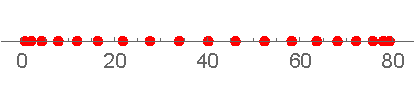
\includegraphics{n20}
%			\caption{Spectrum, $n = 20$}
%		}
%		\only<2>{
%			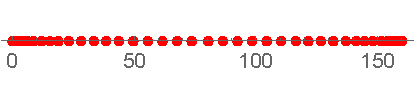
\includegraphics{n40}
%			\caption{Spectrum, $n = 40$}
%		}
%		\only<3>{
%			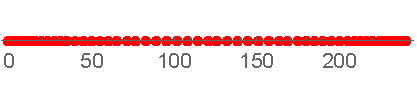
\includegraphics{n60}
%			\caption{Spectrum, $n = 60$}
%		}
%		\end{figure}
%	\end{frame}
%
%	\begin{frame}{The problem with clustering}
%		\textbf{Why simple iterations are not efficient}:
%		\begin{itemize}
%			\item Good at eliminating oscillating components of the error, yet terrible at smooth
%			\item So you may need~$\gg n$ iterations to converge 
%		\end{itemize}
%		\textbf{Why Krylov solvers are not efficient}:
%		\begin{itemize}
%			\item CG:~$|| \vect e_k ||_{\vect A} \le 2 \left( \frac{1 - \sqrt{\kappa^{-1}(\vect A)}}{1 + \sqrt{\kappa^{-1}(\vect A)}} \right)^k || \vect e_0 ||_{\vect A} = 2 \rho^k || \vect e_0 ||_{\vect A}$
%			\item $O(h^{-2}) = \kappa(\vect A) \to \infty$, so~$\rho \to 1$. This is a pessimistic bound, however, it is the case for bad-clustered spectrum
%			\item Thus you will need $n$ iterations (and hence~$O(n^2)$ operations) to converge
%		\end{itemize}
%	\end{frame}
%
%	\begin{frame}{The problem with clustering: CG}
%		\begin{figure}
%			\begin{subfigure}{.5\linewidth}
%				\centering
%				\svginputw[.8]{cg.pdf_tex}
%			\end{subfigure}%
%			\begin{subfigure}{.5\linewidth}
%				CG error norm history, $n = 500$. \textcolor{Blue}{Blue}: ``clustered'' Poisson matrix; \textcolor{Orange}{Orange}: uniform spectrum with cond number as for Poisson; \textcolor{Green}{Green}: uniform spectrum w/ two outliers, $\lambda_1$ and $\lambda_{500}$, s.t. the cond number is 100 times bigger than for Poisson
%			\end{subfigure}
%		\end{figure}
%		Note that (\textcolor{Green}{Green}) after several iterations CG starts to behave like extreme eigenvalues are not present~[1]
%	\end{frame}
%	
%	\section{Diffusion-reaction problem}
%	
%	\begin{frame}{Model problem}
%		We consider diffusion-reaction problem
%		\begin{empheq}[left=\empheqlbrace]{align*}
%			-\epsilon \, \Delta u + u						&= f,		& \vect x & \in \Omega,		& \\
%			u												&= g_D,		& \vect x & \in \Gamma_D,	& \\		
%			\epsilon \, \nabla u \cdot \hat{\vect n} + u	&= g_R,		& \vect x & \in \Gamma_R	&	
%		\end{empheq}
%		\begin{figure}
%			\centering
%			\includegraphicsw[.4]{divgrad_u.png}
%			\caption{Exact solution}
%		\end{figure}
%	\end{frame}
%
%	\begin{frame}{Linear solvers comparison (1\,/\,2)}
%		\begin{table}
%			\centering
%			\caption{
%				Iterations / time ($\|\vect r_i\|/\|\vect r_0\| < 10^{-12}$) as one refines the mesh, $\Omega_1 \subset \Omega_2 \subset \dots \subset \Omega_8$
%			} 
%			\label{tab:divgrad_iters}
%			\footnotesize
%			\begin{tabular}[1.2]{ c c c | c | c | c | c | }
%				& & \multicolumn{5}{c}{\textbf{solver type}} \\ 
%				\cline{3-7}
%				& & \multicolumn{1}{|c|}{MG(V)} & MG(W) & $\Pmgv$CG & $\Pilu$CG & CG \\
%				\cline{2-7} 
%				\multirow{8}{*}{\rotatebox[origin=c]{90}{\textbf{mesh level}}} 
%				& \multicolumn{1}{|c|}{$\Omega_1$} & 8\,/\,.025\,s  & 8\,/\,.018\,s  & 6\,/\,.024\,s & 16\,/\,.032\,s & 37\,/\,.007\,s   \\
%				\cline{2-7}
%				& \multicolumn{1}{|c|}{$\Omega_2$} & 9\,/\,.029\,s  & 9\,/\,.034\,s  & 7\,/\,.032\,s & 28\,/\,.033\,s & 72\,/\,.024\,s   \\
%				\cline{2-7}
%				& \multicolumn{1}{|c|}{$\Omega_3$} & 10\,/\,.035\,s & 9\,/\,.050\,s  & 8\,/\,.045\,s & 53\,/\,.039\,s & 139\,/\,.031\,s  \\
%				\cline{2-7}
%				& \multicolumn{1}{|c|}{$\Omega_4$} & 10\,/\,.079\,s & 10\,/\,.111\,s & 8\,/\,.077\,s & 103\,/\,.064\,s & 276\,/\,.140\,s  \\
%				\cline{2-7}
%				& \multicolumn{1}{|c|}{$\Omega_5$} & 11\,/\,.222\,s & 10\,/\,.385\,s & 8\,/\,.244\,s & 206\,/\,.267\,s & 546\,/\,.859\,s  \\
%				\cline{2-7}
%				& \multicolumn{1}{|c|}{$\Omega_6$} & 11\,/\,.864\,s & 10\,/\,1.09\,s & 8\,/\,.826\,s & 399\,/\,4.49\,s & 1036\,/\,6.30\,s \\
%				\cline{2-7}
%				& \multicolumn{1}{|c|}{$\Omega_7$} & 11\,/\,3.90\,s & 11\,/\,5.33\,s & 8\,/\,2.86\,s & 776\,/\,47.5\,s & 2033\,/\,73.9\,s \\
%				\cline{2-7}
%				& \multicolumn{1}{|c|}{$\Omega_8$} & 11\,/\,16.1\,s & 11\,/\,20.0\,s & 8\,/\,12.9\,s & 1498\,/\,360\,s & 3915\,/\,605\,s \\
%				\cline{2-7}
%			\end{tabular}
%		\end{table}
%	\end{frame}
%
%	\begin{frame}{V-cycle visualization}
%		\begin{figure}[t!]\tiny
%			\centering
%			\begin{subfigure}{.24\linewidth}
%				\includegraphicsw{x_bar.pdf}
%			\end{subfigure}
%			\par\bigskip
%			\begin{subfigure}{.24\linewidth}
%				\includegraphicsw{x_initial.pdf}
%				\caption{$P_h\,\vect x_{\text{initial}}$}
%				\label{fig:divgrad_vcycle:a}
%			\end{subfigure}
%			\hfill
%			\begin{subfigure}{.24\linewidth}
%				\includegraphicsw{x_ssor1.pdf}
%				\caption{$P_h\,\vect x_{\text{presmooth}}$}
%				\label{fig:divgrad_vcycle:b}
%			\end{subfigure}
%			\hfill
%			\begin{subfigure}{.48\linewidth}
%				\begin{subfigure}{.48\linewidth}
%					\includegraphicsw{x_corrected.pdf}
%					\caption{$P_h\,\vect x_{\text{corrected}}$}
%					\label{fig:divgrad_vcycle:c}
%				\end{subfigure}
%				\hfill
%				\begin{subfigure}{.48\linewidth}
%					\includegraphicsw{x_postsmoothed.pdf}
%					\caption{$P_h\,\vect x_{\text{postsmooth}}$}
%					\label{fig:divgrad_vcycle:d}
%				\end{subfigure}
%				\par\bigskip
%				\begin{subfigure}{.48\linewidth}
%					\includegraphicsw{x_ssor2.pdf}
%					\caption{$P_h\,\vect x_{\text{SSOR\,2}}$}
%					\label{fig:divgrad_vcycle:e}
%				\end{subfigure}
%				\hfill
%				\begin{subfigure}{.48\linewidth}
%					\includegraphicsw{x_ssor3.pdf}
%					\caption{$P_h\,\vect x_{\text{SSOR\,3}}$}
%					\label{fig:divgrad_vcycle:f}
%				\end{subfigure}
%			\end{subfigure}
%		\end{figure}
%	\end{frame}
%
%	\begin{frame}{Linear solvers comparison (2\,/\,2)}
%		\begin{figure}
%			\centering
%			\includegraphicsw[.8]{divgrad_time}
%			\caption{}
%		\end{figure}
%	\end{frame}
%
%	\begin{frame}{Convergence for different finite elements}
%		\begin{table}\centering
%			\caption{
%				Linear~(\subref{tab:divgrad_conv:a}), quadratic Lagrange~(\subref{tab:divgrad_conv:b}), and Crouzeix\,--\,Raviart FE~(\subref{tab:divgrad_conv:c}); $i \coloneqq$ mesh level, $e_h \coloneqq \sqrt{\int_{\Omega_h} (u - u_h)^2 \diff{\vect x}}$
%			} 
%			\label{tab:divgrad_conv}
%			\tiny
%			\begin{subtable}[b]{.35\linewidth}
%				\centering
%				\begin{tabular}[.7]{ | c | c | c | }
%					\hline
%					$i$ & $e_i$ & $e_{i-1} / e_i$ \\
%					\hline\hline
%					0	& $7.12 \times 10^{-2}$ & --- \\
%					\hline
%					1	& $2.08 \times 10^{-2}$ & 3.43 \\
%					\hline
%					2	& $5.55 \times 10^{-3}$ & 3.74 \\
%					\hline
%					3	& $1.42 \times 10^{-3}$ & 3.91 \\
%					\hline
%				\end{tabular}
%				\caption{}
%				\label{tab:divgrad_conv:a}
%			\end{subtable}%
%			\begin{subtable}[b]{.3\linewidth}
%				\centering
%				\begin{tabular}[.7]{ | c | c | }
%					\hline
%					$e_i$ & $e_{i-1} / e_i$ \\
%					\hline\hline
%					$8.19 \times 10^{-3}$ & --- \\
%					\hline
%					$1.08 \times 10^{-3}$ & 7.58 \\
%					\hline
%					$1.38 \times 10^{-4}$ & 7.85 \\
%					\hline
%					$1.74 \times 10^{-5}$ & 7.92 \\
%					\hline
%				\end{tabular}
%				\caption{}
%				\label{tab:divgrad_conv:b}
%			\end{subtable}%
%			\begin{subtable}[b]{.3\linewidth}
%				\centering
%				\begin{tabular}[.7]{ | c | c | }
%					\hline
%					$e_i$ & $e_{i-1} / e_i$ \\
%					\hline\hline
%					$5.64 \times 10^{-2}$ & --- \\
%					\hline
%					$1.54 \times 10^{-2}$ & 3.66 \\
%					\hline
%					$3.95 \times 10^{-3}$ & 3.90 \\
%					\hline
%					$9.94 \times 10^{-4}$ & 3.97 \\
%					\hline
%				\end{tabular}
%				\caption{}
%				\label{tab:divgrad_conv:c}
%			\end{subtable}%
%		\end{table} 
%		\begin{figure}
%			\centering
%			\begin{subfigure}{.35\linewidth}\centering
%				\includegraphicsw[.8]{divgrad_l1_u.pdf}
%			\end{subfigure}%
%			\hfill
%			\begin{subfigure}{.3\linewidth}\centering
%				\includegraphicsw[.8]{divgrad_l2_u.pdf}
%			\end{subfigure}%
%			\hfill
%			\begin{subfigure}{.3\linewidth}\centering
%				\includegraphicsw[.8]{divgrad_cr_u.pdf}
%			\end{subfigure}
%			\caption{Corresponding FE solutions~$u_h$}
%			\label{fig:divgrad_solns}
%		\end{figure}
%	\end{frame}
%	
%	\section{Oseen problem}
%	
%	\begin{frame}{Oseen problem}
%		\begin{enumerate}
%			\item After time discretization \& linearization of Navier\,--\,Stokes eqns, one gets
%				\begin{empheq}[left = \empheqlbrace]{align*}
%					\alert{\alpha} \, \vect u + (\alert{\vect w} \cdot \nabla) \vect u - \text{Re}^{-1}\,\Delta \vect u + \nabla p &= \alert{\vect f}, \\
%					\nabla \cdot \vect u &= 0 \quad \text{\alert{(+ BCs)}}
%				\end{empheq}
%			\only<1>{
%			\item Mixed weak form is
%				\begin{empheq}[box=\widefbox]{equation*}
%					\begin{split}
%					&\text{find trial functions $\langle \vect u, p \rangle\in \USpace \times \PSpace$ such that} \\
%					&\left\{
%					\begin{aligned} 
%					\aForm{\vect u}{\vect v} + \bForm{\vect v}{p} &= \lForm{\vect v}, \\
%					\bForm{\vect u}{q} &= 0
%					\end{aligned} 
%					\right. \\ 
%					&\text{holds for all test functions $\langle \vect v, q \rangle\in \USpace \times \PSpace$}
%					\end{split}
%				\end{empheq}}%
%			\only<2>{
%			\item Going to discrete spaces $\USpace_h$, $\PSpace_h$ leads to
%				\begin{equation*}
%				\adjustlimits 
%				\inf_{q_h \in \PSpace_h} \sup_{\vect v_h \in \USpace_h} \frac{
%					\bForm{\vect v_h}{q_h}
%				}{
%					\|q_h\|_{\LSpace} \|\vect v_h\|_{\left[\HSpace\right]^2}
%				} \geq \beta > 0;
%				\quad
%				\underbrace{
%					\begin{pmatrix}
%					\vect A & \vect B^T \\
%					\vect B & O           
%					\end{pmatrix}
%				}_{\mathbcal A \coloneqq}
%				\begin{pmatrix}
%				\vect\xi \\
%				\vect\eta         
%				\end{pmatrix}
%				=
%				\begin{pmatrix}
%				\vect l \\
%				O        
%				\end{pmatrix} % \eqqcolon \vect b
%				\end{equation*}
%		}
%		\end{enumerate}
%	\end{frame}
%
%	\begin{frame}{Physics-based preconditioning}
%		Consider the block decomposition
%		\begin{equation*}
%		\mathbcal A = \mathbcal{L} \, \mathbcal{D} \, \mathbcal{U} = \begin{pmatrix}
%		\vect I & O \\
%		\vect B \, \vect A^{-1} & \vect I
%		\end{pmatrix}
%		\begin{pmatrix}
%		\vect A & O \\
%		O & \vect S
%		\end{pmatrix}
%		\begin{pmatrix}
%		\vect I & \vect A^{-1} \, \vect B^{T} \\
%		O & \vect I
%		\end{pmatrix},
%		\end{equation*}
%		with $\vect S \coloneqq -\vect B \, \vect A \, \vect B^T$ being a pressure Schur complement. 
%		\vfill
%		Preconditioners:
%		\vfill
%		\begin{columns}
%			\begin{column}{.5\textwidth}
%				\begin{block}{Block-diagonal}
%					\begin{equation*}
%					\Pbd \coloneqq \widetilde{\mathbcal D^{-1}} = \widetilde{\begin{pmatrix}
%						\mathbf A & O \\
%						O & \mathbf S
%						\end{pmatrix}^{-1}}
%					\end{equation*}
%					\vspace{5pt}
%				\end{block}
%			\end{column}%
%			\begin{column}{.5\textwidth}
%				\begin{block}{Block-triangular}
%					\begin{equation*}
%					\Pbt \coloneqq \widetilde{(\mathbcal D \, \mathbcal U)^{-1}} = \widetilde{\begin{pmatrix}
%						\vect A & \vect B^T \\
%						O & \vect S
%						\end{pmatrix}^{-1}}
%					\end{equation*}
%					\vspace{5pt}
%				\end{block}
%			\end{column}
%		\end{columns}
%		\end{frame}
%	
%		\begin{frame}{Numerical results}
%			\begin{table}\centering
%				\caption{
%					$\Pbd$BiCGStab and $\Pbt$BiCGStab for haemodynamics Stokes problem ($||\vect r_i|| < 10^{-10}$) for Taylor\,--\,Hood FE; numb of d.o.f. for  $\Omega_0$ is 556, and for $\Omega_5$ is 459\,635
%				} 
%				\label{tab:chd_stokes_iters}
%				\begin{tabular}[1.2]{ c c c | c |}
%					& & \multicolumn{2}{c}{\textbf{solver type}} \\ 
%					\cline{3-4}
%					\multirow{6}{*}{\rotatebox[origin=c]{90}{\textbf{mesh level}}} 
%					& & \multicolumn{1}{|c|}{$\Pbd$BiCGStab} & $\Pbt$BiCGStab \\
%					\cline{2-4} 
%					& \multicolumn{1}{|c|}{$\Omega_1$} & 105\,/\,5.05\,s	& 38\,/\,2.71\,s \\
%					\cline{2-4}
%					& \multicolumn{1}{|c|}{$\Omega_2$} & 129\,/\,16.9\,s	& 41\,/\,5.35\,s \\
%					\cline{2-4}
%					& \multicolumn{1}{|c|}{$\Omega_3$} & 113\,/\,56.4\,s	& 43\,/\,20.4\,s \\
%					\cline{2-4}
%					& \multicolumn{1}{|c|}{$\Omega_4$} & 108\,/\,238\,s		& 43\,/\,84.9\,s \\
%					\cline{2-4}
%					& \multicolumn{1}{|c|}{$\Omega_5$} & ---				& 44\,/\,433\,s \\
%					\cline{2-4}
%				\end{tabular}
%			\end{table}
%		\end{frame}
%	
%		\begin{frame}{Solution postprocessing (1\,/\,2)}
%			\begin{figure}
%				\begin{subfigure}{.9\linewidth}
%					\begin{subfigure}{1.\linewidth}\centering
%						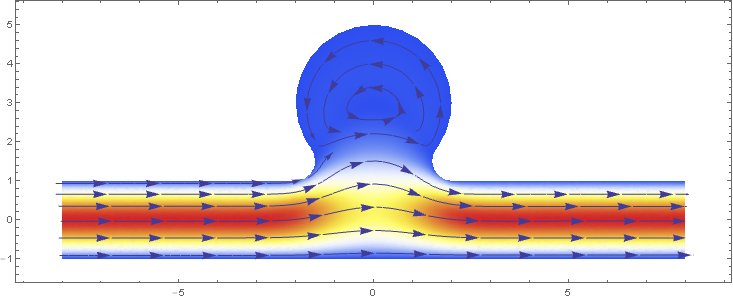
\includegraphics[height=70bp]{chd_u_0.png}\quad
%						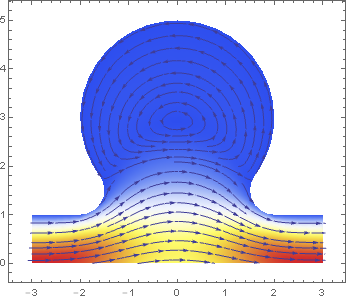
\includegraphics[height=70bp]{chd_u_0_zoom.png}
%					\end{subfigure}%
%					\par\bigskip
%					\begin{subfigure}{1.\linewidth}\centering
%						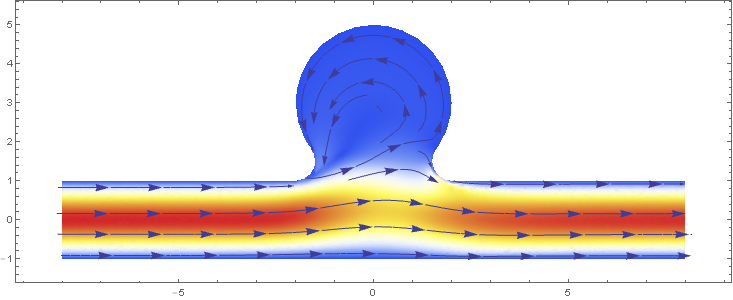
\includegraphics[height=70bp]{chd_u_1.png}\quad
%						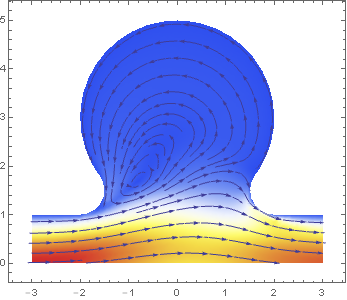
\includegraphics[height=70bp]{chd_u_1_zoom.png}
%					\end{subfigure}%
%				\end{subfigure}%
%				\begin{subfigure}{.1\linewidth}\centering
%					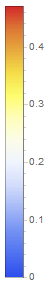
\includegraphics[height=100bp]{chd_u_bar.png}
%				\end{subfigure}%
%				\caption{
%					Velocity fields for Stokes ($t = 0$) and Oseen ($t = 0 + \Delta t = .01$) problems
%				}
%				\label{fig:chd_u}
%			\end{figure}
%		\end{frame}
%		
%		\begin{frame}{Solution postprocessing (2\,/\,2)}
%			\begin{figure}
%			\begin{subfigure}{1.\linewidth}\centering
%				\includegraphicsw[.7]{chd_p_0.png}
%			\end{subfigure}%
%			\par\bigskip
%			\begin{subfigure}{1.\linewidth}\centering
%				\includegraphicsw[.7]{chd_p_1.png}
%			\end{subfigure}
%			\caption{Pressure distributions for Stokes ($t = 0$) and Oseen ($t = 0 + \Delta t = .01$) problems}
%			\label{fig:chd_p}
%			\end{figure}
%		\end{frame}
%	
%	\begin{frame}{Useful references}
%	\begin{enumerate}
%		\item \textbf{General theory}: M.\,Olshanskii \& E.\,Tyrtyshnikov ``Iterative methods for linear systems'' 
%		\item \textbf{Numerical examples with geometric MG}: K.\,Mardal et. al. ``Software tools for multigrid methods''
%		\item \textbf{Physics-based (or block) preconditioners}: \href{https://www.math.colostate.edu/~bangerth/videos.676.38.html}{Woflgang Bangerth's lecture} 
%	\end{enumerate}
%	\end{frame}

\end{document}


